\begin{Exercise}[title=(*)Enroulement d'un fil sur un cylindre]
	\begin{tabular}{cc}
		\begin{minipage}{.5\linewidth}
	Un cylindre de révolution, d’axe vertical, de rayon	R,	repose sur un plan horizontal et fixe par rapport	à un référentiel$(O,\vec{x},\vec{y},\vec{z})$.On attache une extrémité d’un fil parfaitement souple,	infiniment mince et de masse négligeable à la base du cylindre, et on l’enroule plusieurs fois dans le sens trigonométrique autour de cette base.
L’autre extrémité du fil est fixée à une particule $M$
de masse $m$,astreinte à glisser sans frottement sur le plan horizontal.La partie non enroulée du fil est tendue.
\emph{Donnée : $R=$\SI{0.2}{m} ; $m=$\SI{0.04}{kg}; $l_0=I_0M = $\SI{0.5}{m}; $v_0 = $\SI{0.1}{\m\per\s}}
		\end{minipage} &
	\begin{minipage}{.4\linewidth}
	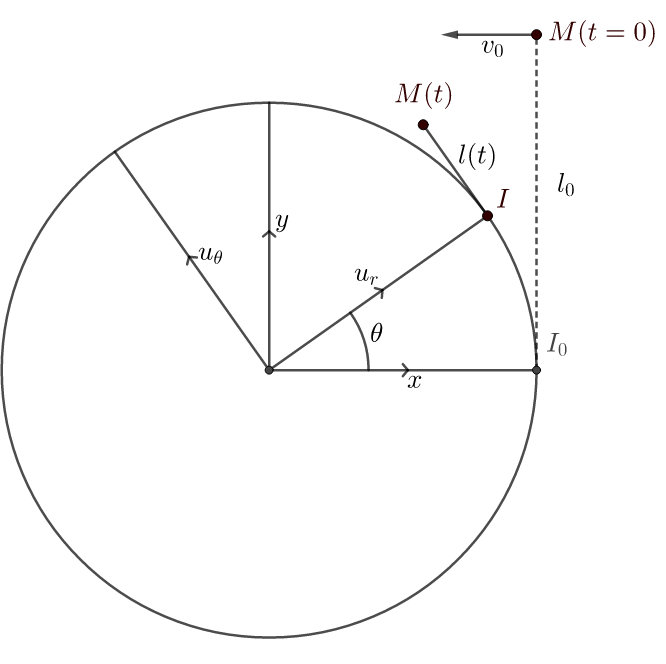
\includegraphics[width=\textwidth]{../fig/Cylindre.png}
	\end{minipage}
	\end{tabular}

	\Question À l’instant t = 0 , on communique à la particule M une vitesse$ \vec{v_0}$ horizontale perpendiculaire à  $I_0M$ et orientée comme l’indiquent la figure ci dessus.
	\Question Exprimer les composantes de $\vec{OM}$ dans le repère $(\vec{u_r} , \vec{u_\theta})$ en fonction de $l_0,R,\theta$.
	\Question En déduire les composantes de la vitesse $\vec{v}$ de la particule $M$ suivant les vecteurs $\vec{u_r}$ et $\vec{u_\theta}$
	\Question Montrer que la norme $v$ de la vitesse reste constante au cours du mouvement.
	\Question Déduire des question précédente une équatio différentielle vérifiée par $\theta$
	\Question Résoudre cette équation différentielle.
	\Question Déterminer $t_f$ instant ou le fil est entièrement enroulé.Application numérique.
	\Question
	\subQuestion Déterminer la tension T du fils en fonction de $t,m,l_0,R, v_0$
	\subQuestion En réalité il y a rupture du fil dès que sa tension dépasse la valeur $T_{rup} =$\SI{5e-3}{N}. Déterminer l'instant $t_r$ et l'angle $\theta_r$ lorsque intervient la rupture du fil. Effectuer l'application numérique.
\end{Exercise}
\begin{Answer}
	\Question $l = l_0 - R\theta$
	\Question $\vec{OM} = \vec{OI}+\vec{IM}=R\vec{u_r}+(l_0-R\theta)\vec{u_\theta}$
	\Question $\vec{v}=-\dot{\theta}(l_0-R\theta)\vec{u_r}$
	\Question On a le poids/réaction (verticale ,pas pris en compte) et la tension $\vec{T}=-T\vec{u_\theta}$ est perpendiculaire à $\vec{v}$ d'ou: $m\dd{\vec{v}}{t}=-T\vec{u_\theta}$ puis: $\vec{v}.\dd{\vec{v}}{t}=0$ donc $v=cst$
	\Question $v_0 = \dot{\theta}(l_0-R\theta)$
	\Question on integre par séparation des variables: $l_0\theta - R\theta^2=v_0t$ donc
	$\boxed{\theta(t)=\frac{l_0}{R}\left(1-\sqrt{1-\frac{2Rv_0t}{l_0^2}}\right)}$
	( car on veux $\theta(t)$ croissant
	\Question $t_f=$\SI{6.25}{s}
	\Question \subQuestion PFD sur $\vec{u_\theta}$ alors :$T=mv_0\dot{\theta}$ donc :
	$\boxed{T= \frac{mv_0^2}{l_0} \left(1-\frac{2Rv_0t}{l_0^2}\right)^{-1/2}}$
	\subQuestion $t_r=$ 6.09 s ; $\theta_r=$\SI{120}{\deg}.
\end{Answer}
